%%%%%%%%%%
% Relatório de Projeto Final - Detecção de Patologias Cardíacas
% Universidade Federal de São Carlos
% Departamento de Ciência da Computação
%%%%%%%%%%

\documentclass[conference]{IEEEtran}

\usepackage[utf8]{inputenc}       
\usepackage[T1]{fontenc}           
\usepackage[brazil]{babel}         
\usepackage{graphicx}              
\usepackage{amsmath, amssymb}      
\usepackage{booktabs}              
\usepackage{caption}              
\usepackage{subcaption}            
\usepackage{hyperref}             

\begin{document}

% Título e Autores

\title{Detecção de Patologias Cardíacas em Pacientes Pediátricos}

\author{
    \IEEEauthorblockN{João Vitor Averaldo Antunes - 813979} 
    \IEEEauthorblockA{
        Universidade Federal de São Carlos (UFSCar) \\
        Bacharelado em Ciência da Computação \\
        18052-780, Sorocaba, São Paulo, Brasil \\
        joaoaveraldo@estudante.ufscar.br
    }
}

\maketitle

% Resumo e Palavras-chave

\begin{abstract}
A detecção precoce de patologias cardíacas em pacientes pediátricos é de extrema importância para a melhoria do prognóstico e para o estabelecimento de tratamentos eficazes. Este trabalho utiliza uma base de dados real, oriunda do Real Hospital Português, contendo registros de crianças, adolescentes e alguns dados adultos, para treinar modelos de aprendizado de máquina visando a predição da presença de patologias. São exploradas técnicas de pré-processamento, incluindo tratamento de outliers, padronização de variáveis e codificação de variáveis categóricas, ajuste de hiperparâmetros via GridSearchCV e avaliação de modelos (KNN, Naïve Bayes, Regressão Logística, MLP, SVM e RandomForest) com métricas como acurácia, precisão, recall, F1-Score e ROC-AUC. Os resultados indicam que o modelo RandomForest alcança o melhor desempenho em ROC-AUC, demonstrando robustez e adequação para a tarefa proposta.
\end{abstract}

\begin{IEEEkeywords}
Patologias cardíacas, pacientes pediátricos, aprendizado de máquina, análise exploratória, pré-processamento, experimentos, análise de resultados.
\end{IEEEkeywords}

% I. Introdução

\section{Introdução}
O diagnóstico precoce de patologias cardiovasculares em crianças é um dos maiores desafios na prática clínica, principalmente devido à natureza assintomática de muitas dessas condições durante suas fases iniciais. Essa dificuldade muitas vezes impede a identificação e o tratamento oportuno, aumentando o risco de complicações futuras. Em um cenário onde a saúde infantil demanda intervenções rápidas e precisas, a aplicação de técnicas de aprendizado de máquina surge como uma ferramenta promissora, capaz de analisar grandes volumes de dados clínicos e auxiliar os profissionais de saúde na tomada de decisão.

Neste trabalho, foi explorada uma base de dados real, coletada no Real Hospital Português (RHP). Além disso, a base abrange registros de pacientes com até 19 anos, além de um número reduzido de dados de adultos, assim como contém diversas variáveis clínicas relevantes, como pressão arterial, idade, peso, altura, IMC e variáveis derivadas — por exemplo, a Pressão de Pulso Arterial e os motivos que levaram os pacientes à busca por avaliação médica.

O objetivo central deste estudo é investigar a viabilidade de empregar modelos de aprendizado de máquina na detecção precoce de potenciais problemas cardíacos em pacientes pediátricos. Pretende-se, com isso, identificar padrões e indicadores que possam, futuramente, colaborar para a definição de estratégias preventivas e para o aprimoramento do diagnóstico clínico. Desse modo, ao conduzir uma análise detalhada e um rigoroso processo de pré-processamento dos dados, este trabalho busca demonstrar que a integração entre informações clínicas reais e técnicas de aprendizado de máquina pode resultar em ferramentas valiosas para o apoio à decisão médica.

Portanto, este estudo não tem relevância apenas na área tecnológica e matemática, mas também na perspectiva de melhorar a qualidade do atendimento e a saúde das crianças, no intuito de contribuir para avanços na área médica


% II. Trabalhos Relacionados

\section{Trabalhos Relacionados}
Diversos estudos têm se dedicado à aplicação de técnicas de aprendizado de máquina para a detecção de anomalias e patologias em bases de dados clínicas, ressaltando a importância de um pré-processamento robusto e do ajuste fino dos hiperparâmetros para a obtenção de resultados satisfatórios. Assim sendo, a utilização de modelos preditivos para o diagnóstico de hipertensão em crianças requer a aplicação rigorosa de protocolos de medição e interpretação dos dados clínicos, pois os parâmetros variam significativamente conforme a idade, o sexo e a estatura \cite{ref:Araujo2024}. 

Além disso, a padronização das medidas de pressão arterial, de acordo com as diretrizes nacionais, é fundamental para garantir a qualidade dos dados e, consequentemente, a acurácia dos modelos de aprendizado de máquina \cite{ref:Feitosa2024}. Ademais, algoritmos bem calibrados, quando treinados com dados corretamente normalizados e ajustados, são capazes de identificar padrões relevantes para a detecção precoce de alterações cardiovasculares \cite{ref:Goodfellow2016}.

Adicionalmente, estudos demonstram que a pressão de pulso é um marcador importante de risco, reforçando a necessidade de incluir variáveis que reflitam a dinâmica arterial nos modelos preditivos \cite{ref:Vasan2002}. De forma complementar, pesquisas realizadas em ambientes hospitalares indicam que a integração de dados de sinais vitais de diferentes faixas etárias pode aprimorar a generalização dos modelos preditivos \cite{ref:Islam2024}.

A abordagem deste trabalho combina dados pediátricos e adultos, utilizando os dados dos adultos para auxiliar no treinamento dos modelos. Essa estratégia permite ampliar o volume de dados e melhorar a representatividade dos padrões fisiológicos, contribuindo para a robustez e a eficácia dos algoritmos empregados na detecção de anomalias.

% III. Dados e Pré-processamento

\section{Dados e Pré-processamento}
A base de dados utilizada contém informações detalhadas de variáveis clínicas essenciais, obtidas de registros do RHP e da Universidade do Porto. As principais etapas da análise exploratória, isto é, a identificação da variedade de dados e dos focos de mudanças e do consequente pré-processamento foram:

\subsection{Análise Exploratória}
\begin{itemize}
    \item \textbf{Matriz de Correlação:} \\
    \begin{figure}[ht]
        \centering
        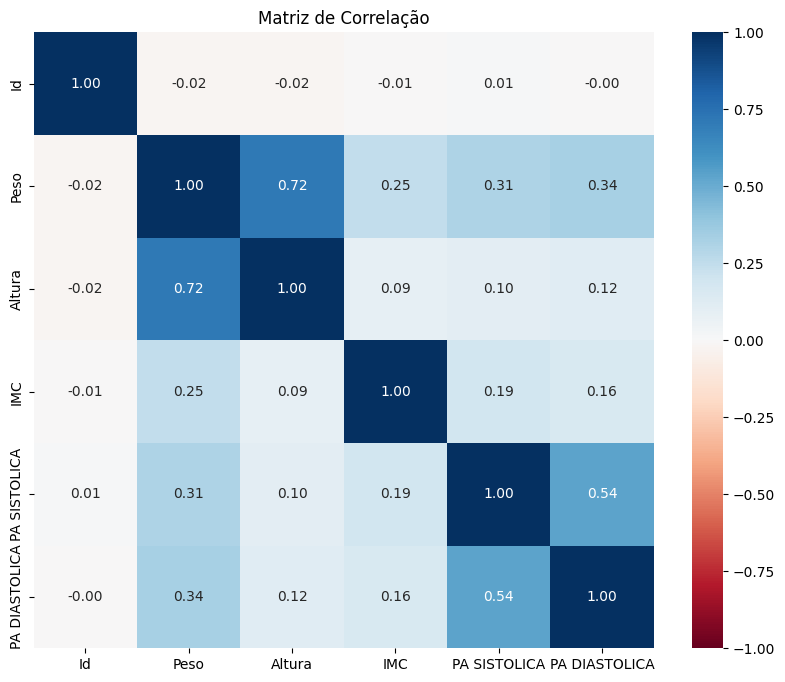
\includegraphics[width=0.45\textwidth]{matriz_correlacao.png}
        \caption{Matriz de Correlação dos atributos numéricos}
        \label{fig:learning_curve}
    \end{figure}
    
    A partir de uma análise sob a Matriz de Correlação (Figura 1) dos atributos numéricos, mostrou  que não há variáveis com correlação extremamente alta (valores superiores a 0,9), o que sugere que não há atributos redundantes a serem removidos. Os valores mais altos foram dos atributos Peso e Altura, com 0.72. \\
 
    \item \textbf{Gráficos Boxplot:} \\
    \begin{figure}[ht]
        \centering
        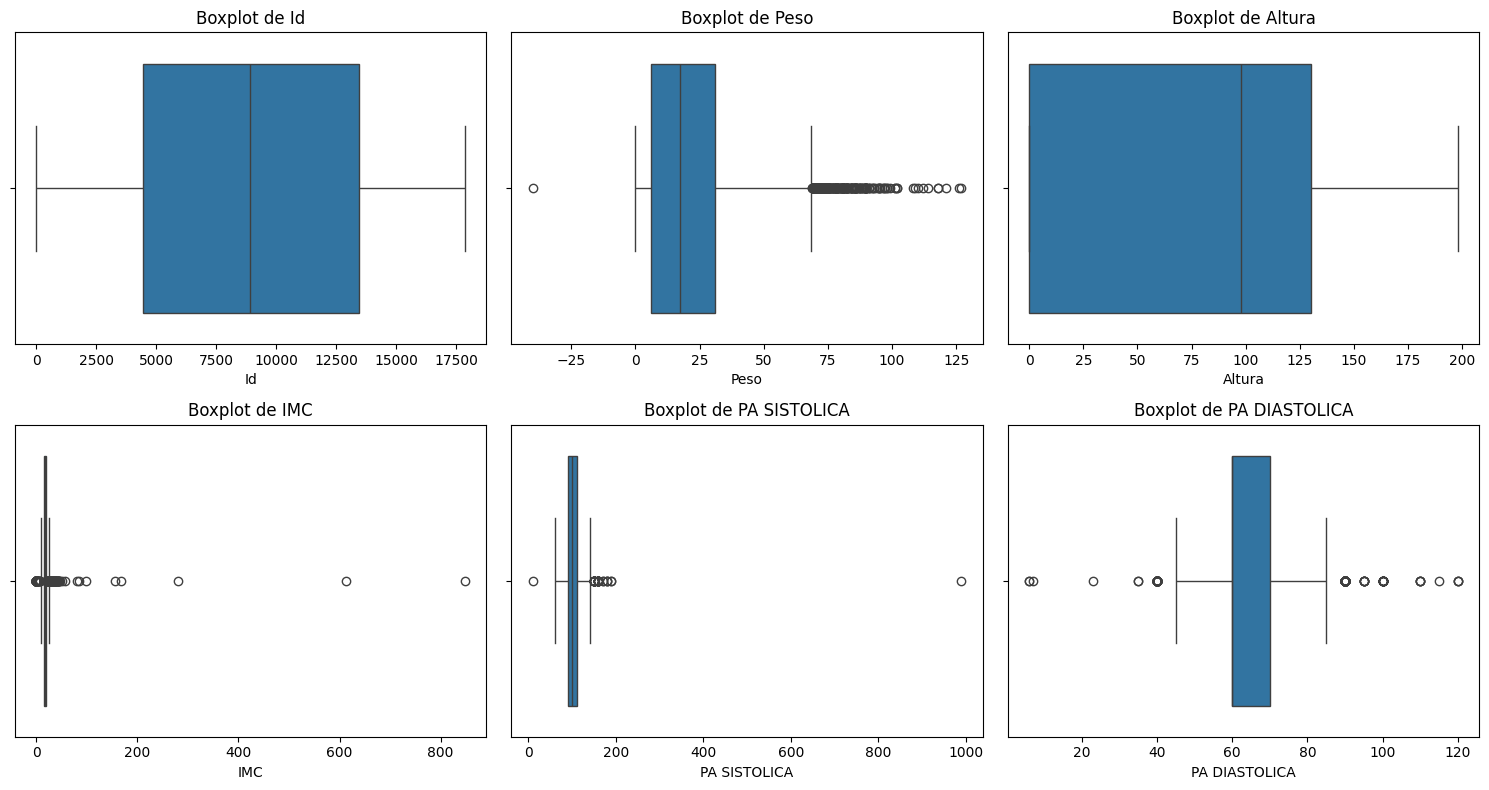
\includegraphics[width=0.45\textwidth]{boxplots.png}
        \caption{Gráficos Boxplot dos atributos numéricos}
        \label{fig:boxplots}
    \end{figure}
    
    Além disso, através da análise dos gráficos Boxplot (Figura 2) foi possível não apenas notar a presença de outliers e valores negativos (que foram tratados de maneira personalizada, conforme o mais adequado para cada coluna), como também notar a ausência de valores que poderiam ser classificados como numéricos, tal qual a Frequência Cardíaca.\\
    
    \item \textbf{Histogramas:} \\
    \begin{figure}[ht]
        \centering
        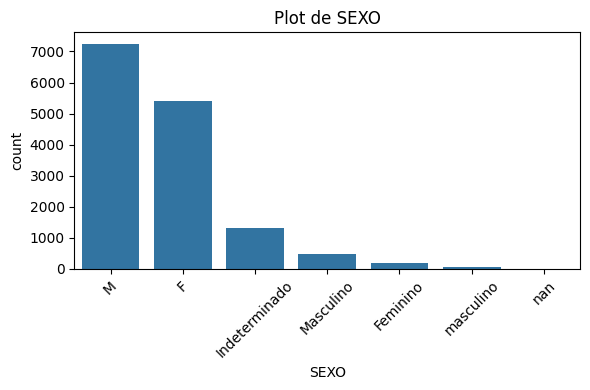
\includegraphics[width=0.45\textwidth]{hist_sexo.png}
        \caption{Histograma dos valores presentes na coluna 'Sexo'}
        \label{fig:hist_sexo.png}
    \end{figure}
    
    Por fim, foram gerados histogramas para todas as colunas, possibilitando visualizar a distribuição dos valores preenchidos. Inicialmente, devido à grande variedade de valores o histograma serve apenas como uma base auxiliar, detectando pontuais mudanças necessárias, como a necessidade de padronização de valores categóricos, notável ao analisar o histograma da coluna 'Sexo' (Figura 3), o qual possui diferentes categorizações para o mesmo valor.
\end{itemize}

\subsection{Tratamento de Dados}
Conforme o modelo se desenvolveu e através de materiais relevantes para o escopo do projeto, foi possível identificar formas coesas de tratar os dados, lidando com cada coluna de forma específica.
\begin{itemize}
    \item \textbf{Classe:} Foi realizada a alteração dos rótulos (por exemplo, renomeação de “anormais”) e remoção de tuplas sem classe, garantindo a qualidade e a padronização dos dados.
    \item \textbf{Datas e Idade:} As colunas referentes à data de atendimento e data de nascimento foram convertidas para o formato \texttt{datetime}. A idade foi recalculada com base nas datas, e valores fora do intervalo (0 $\leq$ x $<$ 120) foram ajustados pela média, preservando ainda os dados de adultos para auxiliar no treinamento.
    \item \textbf{Variáveis Irrelevantes:} Colunas como convênio, data de nascimento, data de consulta e PPA foram removidas, pois não agregam valor ao modelo.
    \item \textbf{Tratamento Específico de Variáveis:}
    \begin{itemize}
        \item \emph{Pulsos e Sopro:} Padronização dos diferentes valores através de um mapeamento para valores únicos.
        \item \emph{FC:} Valores representados como intervalos foram substituídos pela média. 
        \item \emph{Peso e Altura:} Valores considerados fora do intervalo possível foram corrigidos (por exemplo, peso igual a 0 -> mediana ou altura menor que 25 cm -> mediana); 
        \item \emph{PA Sistólica e Diastólica:} Pressões fora dos intervalos (PA sistólica: 40--200; PA diastólica: 40--120) foram ajustadas \cite{ref:ESC2018}.
        \item \emph{IMC:} Recalculado com base nos valores corrigidos de peso e altura.
        \item \emph{Sexo:} Padronização para as categorias \emph{Masculino}, \emph{Feminino} e \emph{Indeterminado}.
    \end{itemize}
    \item \textbf{Codificação e Normalização:} As variáveis categóricas foram codificadas utilizando \emph{one-hot encoding} em vez do \emph{label}, dado que evita atribuir uma ordem arbitrária às categorias, o que poderia estar induzindo o modelo a interpretar relações inexistentes entre elas. Enquanto as variáveis numéricas foram normalizadas pelo método \emph{standard}, preservando a distribuição original sem comprimir excessivamente os valores extremos, ao contrário do \emph{MinMax} ou do \emph{Robust} que podem distorcer as diferenças entre os valores.
    \item \textbf{Tratamento de Valores Nulos:} A substituição dos NaNs em colunas numéricas foi realizada majoritariamente pela média, tendo sido observado um desempenho ligeiramente superior à mediana na maioria dos casos. Paralelamente, para as colunas categóricas a substituição deu-se através da moda (\emph{most\_frequent}) dos valores do atributo em questão.
\end{itemize}

% IV. Protocolo Experimental

\section{Protocolo Experimental}
O fluxo experimental adotado para o treinamento foi baseado em testagens práticas e na pesquisa de boas práticas e convenções para cada um dos modelos treinados. Dessa forma, a escolha da passagem dos parâmetros, assim como a avaliação dos modelos, seguiu os passos abaixo:

\subsection{PCA dos dados}

\begin{figure}[ht]
    \centering
    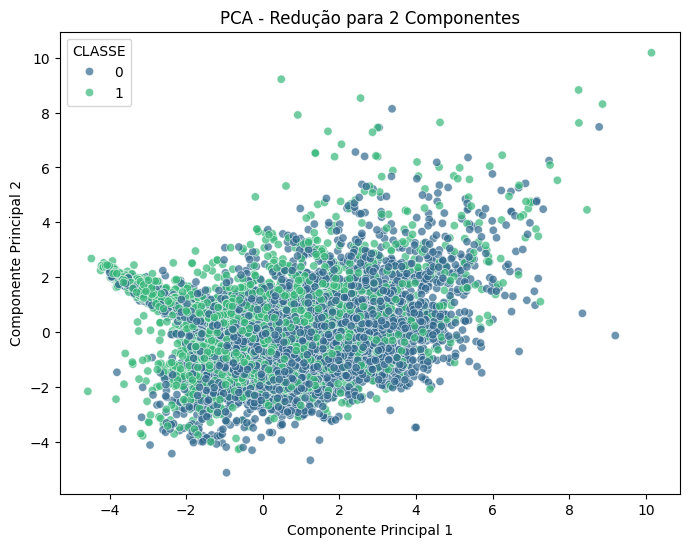
\includegraphics[width=0.35\textwidth]{pca.png}
    \caption{PCA dos dados pré-processados}
    \label{fig:pca}
\end{figure}

A partir da análise do PCA (Figura 4) é perceptível que não há uma separação clara entre as classes. Isso sugere que modelos de classificação mais complexos podem ser necessários para capturar a variabilidade presente nos dados, de forma a distinguir as classes de maneira eficaz.

\subsection{Escolha dos Parâmetros dos Modelos}

\subsubsection{KNN}
\textbf{Parâmetros escolhidos:}

\texttt{\{'n\_neighbors': [3, 5, 7, 9], 'weights': ['uniform', 'distance']\}}.  

Valores menores de \texttt{n\_neighbors} permitem capturar variações locais, enquanto valores maiores suavizam a fronteira de decisão, ajudando na generalização. A ponderação por distância (\texttt{'distance'}) ajusta a influência das amostras vizinhas de forma mais precisa, o que pode melhorar o desempenho do classificador \cite{ref:knn}.

\subsubsection{Naïve Bayes}
Modelo utilizado com os parâmetros padrão.  

Devido à natureza probabilística do Naïve Bayes e sua simplicidade, os parâmetros padrão geralmente apresentam desempenho satisfatório sem a necessidade de ajustes, conforme evidenciado em \cite{ref:NB}.

\subsubsection{Regressão Logística}
\textbf{Parâmetros escolhidos:} 

\texttt{\{'C': [0.01, 0.1, 1, 10, 100], 'solver': ['lbfgs', 'liblinear']\}}.  
 
O parâmetro \texttt{C} controla a regularização, onde valores menores aumentam a penalidade contra coeficientes grandes, prevenindo overfitting, e valores maiores permitem modelos mais flexíveis. A escolha de diferentes solvers possibilita encontrar a melhor otimização para o conjunto de dados, conforme discutido em \cite{ref:logistic}.

\subsubsection{MLP}
\textbf{Parâmetros escolhidos:} 

\texttt{\{'hidden\_layer\_sizes': [(100,), (50,50), (100,50)], 'activation': ['relu', 'tanh']\}}.  
 
As diferentes camadas ocultas permitem testar a capacidade do modelo em capturar padrões. As funções de ativação ReLU e Tanh foram escolhidas por sua eficácia em problemas não-lineares, conforme evidenciado em \cite{ref:mlp}.

\subsubsection{SVM}
\textbf{Parâmetros escolhidos:} 

\texttt{\{'C': [0.1, 1, 10], 'kernel': ['linear', 'rbf']\}}.  

O parâmetro \texttt{C} equilibra a margem de separação e o erro de classificação. Ademais, a utilização dos kernels linear e RBF permite avaliar tanto uma separação linear quanto uma modelagem não-linear dos dados. Essas escolhas estão em linha com as recomendações de \cite{ref:svm}.

\subsubsection{RandomForest}
\textbf{Parâmetros escolhidos:} 

    \texttt{\{'n\_estimators': [100, 200, 300], 'max\_depth': [None, 10, 20, 30], 'min\_samples\_split': [2, 5, 10], 'min\_samples\_leaf': [1, 2, 4], 'bootstrap': [True, False]\}}.  
 
O número de árvores (\texttt{n\_estimators}) e a profundidade máxima (\texttt{max\_depth}) afetam a capacidade de captura de padrões complexos e o risco de overfitting. Os parâmetros \texttt{min\_samples\_split} e \texttt{min\_samples\_leaf} controlam a granularidade das divisões e ajudam a reduzir a variância. A opção de bootstrap foi testada para verificar a influência na robustez do modelo. Essas configurações seguem as melhores práticas descritas em \cite{ref:rf}.

\subsection{Avaliação de cada modelo}
    Para cada um dos modelos, a seguinte rotina foi efetuada, buscando os melhores parâmetros e avaliando o modelo mais adequado para classificar o conjunto de dados de teste.
    \begin{itemize}
        \item Realização de ajuste dos hiperparâmetros via \texttt{GridSearchCV}, buscando o melhor conjunto com base na ROC-AUC.
        \item Treinamento do modelo e avaliação utilizando o conjunto de teste (métricas: acurácia, precisão, recall, F1-Score e ROC-AUC).
        \item Validação adicional por meio de validação cruzada, de modo a verificar a possibilidade de \emph{overfitting} ou \emph{underfitting}.
        \item Impressão dos resultados, inclusive com matrizes de confusão e relatórios de classificação.
    \end{itemize}

% V. Resultados e Análise dos Resultados

\section{Resultados e Análise dos Resultados}
Após a execução dos experimentos, os modelos apresentaram os seguintes resultados aproximados (Tabela 1), com o melhor desempenho em relação ao conjunto de dados de testes na plataforma de submissões do Kaggle sendo 0.95175:

\bigskip

\begin{table}[ht]
\centering
\resizebox{\linewidth}{!}{%
\begin{tabular}{lccccc}
\toprule
Modelo & Acurácia & Precisão & Recall & F1-Score & ROC-AUC \\
\midrule
KNN                & 0.9134 & 0.9368 & 0.8201 & 0.8746 & 0.9293 \\
Naïve Bayes        & 0.8527 & 0.9299 & 0.6485 & 0.7641 & 0.9211 \\
LogisticRegression & 0.9297 & 0.9497 & 0.8542 & 0.8995 & 0.9466 \\
MLP                & 0.9199 & 0.9117 & 0.8662 & 0.8884 & 0.9420 \\
SVM                & 0.9297 & 0.9461 & 0.8579 & 0.8999 & 0.9408 \\
RandomForest       & 0.9318 & 0.9482 & 0.8616 & 0.9029 & 0.9541 \\
\bottomrule
\end{tabular}
}
\caption{Métricas de Desempenho por Modelo}
\label{tab:metricas}
\end{table}

\bigskip

\noindent
Observa-se que, o melhor modelo em relação a Acurácia foi o RandomForest (0.9318), para Precisão foi a Regressão Logística (0.9497), de Recall tem-se o MLP (0.8662) com o valor mais alto, o melhor modelo para F1-Score foi o (0.9092) e para o ROC-AUC foi o RandomForest (0.9541). 

Além disso, considerando que o critério de avaliação principal é o valor da área sob a curva ROC, é razoável verificar o desempenho do RandomForest e sua curva de aprendizado (Figura 5). Assim sendo, o modelo demonstrou pontuações de treinamento elevadas, sendo observável uma estabilização em torno de 0.99 para 12.000 exemplos e uma boa generalização (próximo de 0.96 para o conjunto de validação), com uma diferença percentual inferior a 4\verb|%|. Portanto, pode-se considerar que possui baixos indicadores de \emph{overfitting} e \emph{underfitting} \cite{ref:overfit}. 

No entanto, o valor de recall de 0.8616 indica que aproximadamente 14\verb|%| dos pacientes com patologias são classificados como normais, o que é preocupante, pois representa uma lacuna na detecção de condições críticas.

\begin{figure}[ht]
    \centering
    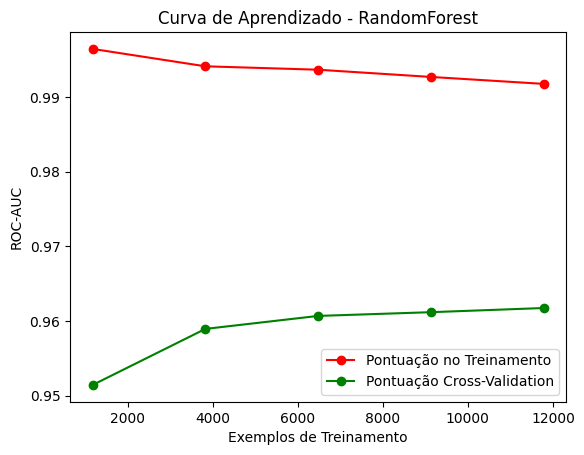
\includegraphics[width=0.45\textwidth]{curva_aprendizado.png}
    \caption{Curva de Aprendizado do Modelo RandomForest}
    \label{fig:curva_aprendizado}
\end{figure}

% VI. Conclusões e Trabalhos Futuros

\section{Conclusões e Trabalhos Futuros}
Neste trabalho, foram aplicadas técnicas de aprendizado de máquina para a detecção precoce de patologias cardíacas em pacientes pediátricos, utilizando uma base de dados real coletada no Real Hospital Português. O rigoroso processo de pré-processamento — que envolveu análise exploratória, tratamento de outliers, normalização e codificação adequada das variáveis — foi fundamental para garantir a qualidade dos dados e, consequentemente, a robustez dos modelos treinados.

Entre os modelos avaliados, o RandomForest obteve a maior área sob a curva ROC (ROC-AUC). Esses resultados ressaltam a importância do ajuste fino dos hiperparâmetros e evidenciam que, embora cada modelo possua suas particularidades, a integração de informações clínicas reais com técnicas de aprendizado de máquina pode gerar ferramentas preditivas eficazes para o apoio à decisão médica.

A análise das curvas de aprendizado revelou que os modelos, em especial o RandomForest, apresentaram boa generalização, com pequenas diferenças entre as pontuações de treinamento e validação. Esse comportamento sugere baixos indicadores de \emph{overfitting} e reforça a confiabilidade dos métodos aplicados. Entretanto, a possibilidade de gerar um número consideravelmente alto de falsos negativos deve ser algo a ser levado em consideração em relação a adoção de modelos como esse.

Como trabalhos futuros, sugerem-se a possibilidade de investigar a inclusão de novos atributos derivados ou variáveis temporais que possam capturar melhor a dinâmica dos sinais vitais e outros parâmetros clínicos. Ademais, pode-se validar os modelos utilizando bases de dados externas, provenientes de outros hospitais, para testar a generalização e a robustez dos algoritmos desenvolvidos.
\end{itemize}

\section*{Agradecimentos}

O autor é grato à estudante de medicina Laura Beani, pelo auxílio na interpretação dos atributos.

% REFERÊNCIAS

\begin{thebibliography}{1}

\bibitem{ref:Araujo2024}
M.~F. Araújo, 
``Use of supervised machine learning to predict arterial hypertension and diabetes mellitus based on sociodemographic and lifestyle data,'' 
Tese (Doutorado em Biotecnologia em Saúde e Medicina Investigativa), Instituto Gonçalo Moniz, Fundação Oswaldo Cruz, Salvador, 2024.

\bibitem{ref:Feitosa2024}
F.~Feitosa \emph{et al.}, 
``Diretrizes Brasileiras de Medidas da Pressão Arterial Dentro e Fora do Consultório – 2023,'' 
\emph{Arq. Bras. Cardiol.}, vol.~121, no.~4, e20240113, 2024.

\bibitem{ref:Goodfellow2016}
I.~Goodfellow, Y.~Bengio, and A.~Courville, 
``Deep Learning,'' 
Cambridge, MA: MIT Press, 2016.

\bibitem{ref:Vasan2002}
R.~S. Vasan, 
``Pulse pressure and cardiovascular disease risk: a review,'' 
\emph{JAMA}, vol.~288, no.~3, pp. 308--316, 2002.

\bibitem{ref:Islam2024}
S.~M.~S. Shariful Islam \emph{et al.}, 
``Machine Learning Models for the Identification of Cardiovascular Diseases Using UK Biobank Data,'' 
arXiv:2407.16721, 2024.

\bibitem{ref:ESC2018}
B. Williams \emph{et al.},
``2018 ESC/ESH Guidelines for the management of arterial hypertension,''
\emph{European Heart Journal}, vol.~39, no.~33, pp. 3021--3104, 2018.

\bibitem{ref:knn}
T. M. Cover and P. E. Hart, 
``Nearest neighbor pattern classification,'' 
\emph{IEEE Transactions on Information Theory}, vol.~13, no.~1, pp. 21--27, 1967.

\bibitem{ref:NB}
H. Zhang,
``The Optimality of Naive Bayes,''
in \emph{Proceedings of the 17th International Florida Artificial Intelligence Research Society Conference}, pp. 1--6, 2004.

\bibitem{ref:logistic}
G. James, D. Witten, T. Hastie, and R. Tibshirani, 
``An Introduction to Statistical Learning: with Applications in R,''
Springer, New York, 2013.

\bibitem{ref:mlp}
Y. LeCun, Y. Bengio, and G. Hinton, 
``Deep learning,'' 
\emph{Nature}, vol. 521, pp. 436--444, 2015.

\bibitem{ref:svm}
C. Cortes and V. Vapnik, 
``Support vector networks,''
\emph{Machine Learning}, vol.~20, no.~3, pp. 273--297, 1995.

\bibitem{ref:rf}
L. Breiman, 
``Random Forests,''
\emph{Machine Learning}, vol. 45, no. 1, pp. 5--32, 2001.

\bibitem{ref:overfit}
T. Hastie, R. Tibshirani, and J. Friedman, 
``The Elements of Statistical Learning: Data Mining, Inference, and Prediction,''
Springer, New York, 2009.

\end{thebibliography}

\end{document}
